\documentclass[12pt]{article}
\usepackage{tikz}
\usetikzlibrary{automata, positioning, arrows}

\title{SE 3310 Theoretical Foundations of Software Engineering Assignment 1}
\author{Marcus Tuen Muk}
\date{January 26 2023}


\begin{document}

    \begin{titlepage}
        \clearpage\maketitle
        \thispagestyle{empty}
    \end{titlepage}

    \section{Identify the regular languages}
        \subsection{\[L_a = \{wwwa^n:w \in \{a,b\}, n > 0\}\]}
            \indent
            Based on this language, w is either all a or all b. This language is a regular language.
            \begin{figure}[ht]
                \centering
                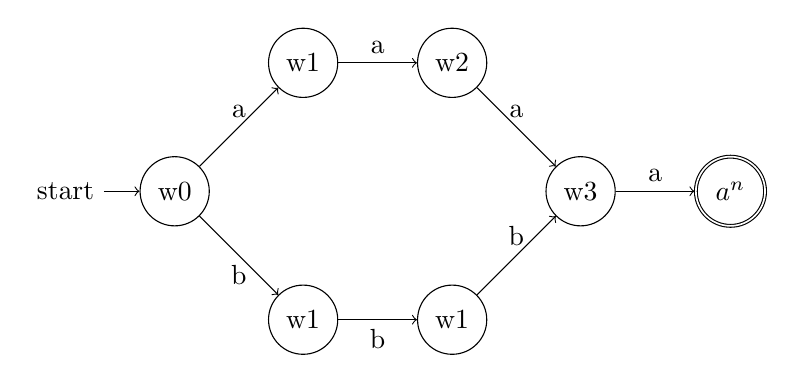
\begin{tikzpicture}
                    \node[state, initial] (w0) {w0};
                    \node[state, above right = of w0] (a1) {w1};
                    \node[state, right = of a1] (a2) {w2};
                    \node[state, below right =of w0] (b1) {w1};
                    \node[state, right =of b1] (b2) {w1};
                    \node[state, below right =of a2] (w3) {w3};
                    \node[state, accepting, right =of w3] (an) {\(a^n\)};
                    

                    \draw   (w0) edge[->, right, above] node{a} (a1)
                            (w0) edge[->, right, below] node{b} (b1)
                            (a1) edge[->, right] node[above] {a} (a2)
                            (b1) edge[->, right] node[below] {b} (b2)
                            (a2) edge[->, right] node[above] {a} (w3)
                            (b2) edge[->, right] node[above] {b} (w3)
                            (w3) edge[->, right] node[above] {a} (an);
                        
                \end{tikzpicture}  
            \end{figure}
        
            \pagebreak
            
            \subsection{\[L_b = \{w \in \{0,1\}*:w \ represents \ as \ a \ binary \ integer \ is \ a \ power \ of \ 4\}\]}
                \indent
                This language is a regular language.
                \begin{figure}[ht]
                    \centering
                    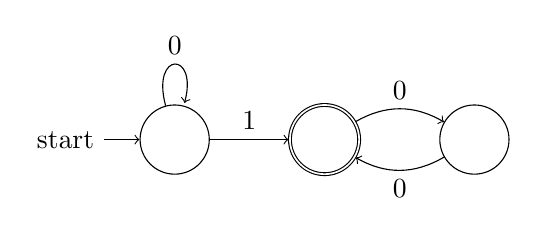
\begin{tikzpicture}
                        \node[state, initial] (w0) {};
                        \node[state, accepting, right = of w0] (w1) {};
                        \node[state, right = of w1] (w2) {};

                        \draw   (w0) edge[->, loop above] node{0} (w0)
                                (w0) edge[->, right] node[above] {1} (w1)
                                (w1) edge[->, bend left] node[above] {0} (w2)
                                (w2) edge[->, bend left] node[below] {0} (w1);
                            
                    \end{tikzpicture}  
                \end{figure}

                \pagebreak

                \subsection{\[L_c = \{wxa: w,x \in \{a,b\}*\}\]}
                \indent
                This language is a regular language.
                \begin{figure}[ht]
                    \centering
                    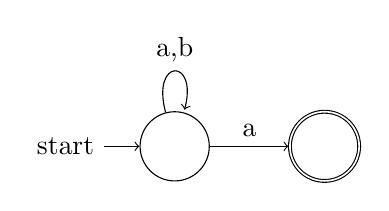
\begin{tikzpicture}
                        \node[state, initial] (wx0) {};
                        \node[state, accepting, right = of wx0] (a) {};

                        \draw   (wx0) edge[->, loop above] node{a,b} (wx0)
                                (wx0) edge[->, right] node[above] {a} (a);
                            
                    \end{tikzpicture}  
                \end{figure}

                \pagebreak

                \subsection{\[L_c = \{wwa: w,x \in \{a,b\}*\}\]}
                \indent
                This language is not a regular language. This language states that some w is a string that
                can be of length 0 or greater and will occur twice. As such, it would need the Finite state
                Machine (FSM) to store the length of w to ensure both strings are the same length. However,
                FSM don't have this capability, thus making this language not a regular language.
                
            \pagebreak 

        \section{Describe the language}
            The formal description of a DFA \emph{M} is given as follows. 
            Let: \[S = \{q_0, q_1, q_2, q_3\}\]
                \[\Sigma = \{a, b, c\}\]
                \[start = q_0\]
                \[F= \{q_3\}\]
            \\ and let $\delta$ be given by the following table:
                \begin{center}
                    \begin{tabular}{ c |c c c}
                         & a & b & c \\ 

                        \hline

                        $q_0$ & $q_1$ & $q_2$ & $q_0$ \\ 
                        $q_1$ & $q_3$ & $q_2$ & $q_2$ \\
                        $q_2$ & $q_1$ & $q_3$ & $q_1$ \\
                        $q_3$ & $q_3$ & $q_3$ & $q_3$ \\  
                    \end{tabular}
                \end{center}
                
            \subsection{Give the state diagram of this machine}
                


\end{document}